\chapter{Manual de usuario}

\section{Visión general}

En este capítulo se muestran los manuales que explican paso a paso cómo hacer uso de las herramientas desarrolladas a nivel de usuario. Los mismos se dividen en dos manuales correspondientes:

\begin{itemize}
	\item \textbf{Manual de usuario del servidor \acrshort{oaipmh}:} este manual abarca todas las posibles consultas que se pueden realizar al servidor mediante un cliente \acrshort{oaipmh} web genérico como puede ser el propio \acrshort{oaipmh} validator.
	\item \textbf{Manual de usuario de la aplicación web:} este manual abarca todos los pasos para realizar las búsquedas avanzadas en proyectos y publicaciones desde el portal web \acrshort{labman}.
\end{itemize}

\section{Manual de usuario del servidor OAI-PMH}

\section{Manual de usuario de la aplicación web}

\subsection{Página principal de LabMan}

Nada más acceder al portal web de \acrshort{labman}, se visualiza su \textit{homepage} (ver figura \ref{fig:morelab_homepage}). En ella se muestra una imagen con los miembros grupo, la descripción y las últimas noticias relacionadas con el equipo de investigación en cuestión.

Por otra parte, se presenta una barra de navegación, con todas las siguientes opciones que ofrece \acrshort{labman} por defecto:

\begin{itemize}
	\item \textbf{News:} Muestra un buscador paginado con el registro \acrfull{rss} de las noticias relacionadas con el equipo de investigación.
	\item \textbf{Projects:} Muestra un buscador paginado con el registro de los proyectos que involucran a los miembros del equipo de investigación.
	\item \textbf{Publications:} Muestra un buscador paginado con el registro de las publicaciones redactadas por los miembros del equipo de investigación.
	\item \textbf{Member:} Muestra la lista con los integrantes del grupo de investigación.
	\item \textbf{Charts:} Muestra el menú por el que se accederán a las gráficas formadas a partir de los datos de los apartados anteriores.
	\item \textbf{About:} Muestra información adicional relacionada con el grupo de investigación.
\end{itemize}

\begin{figure}[!htbp]
	\centering
	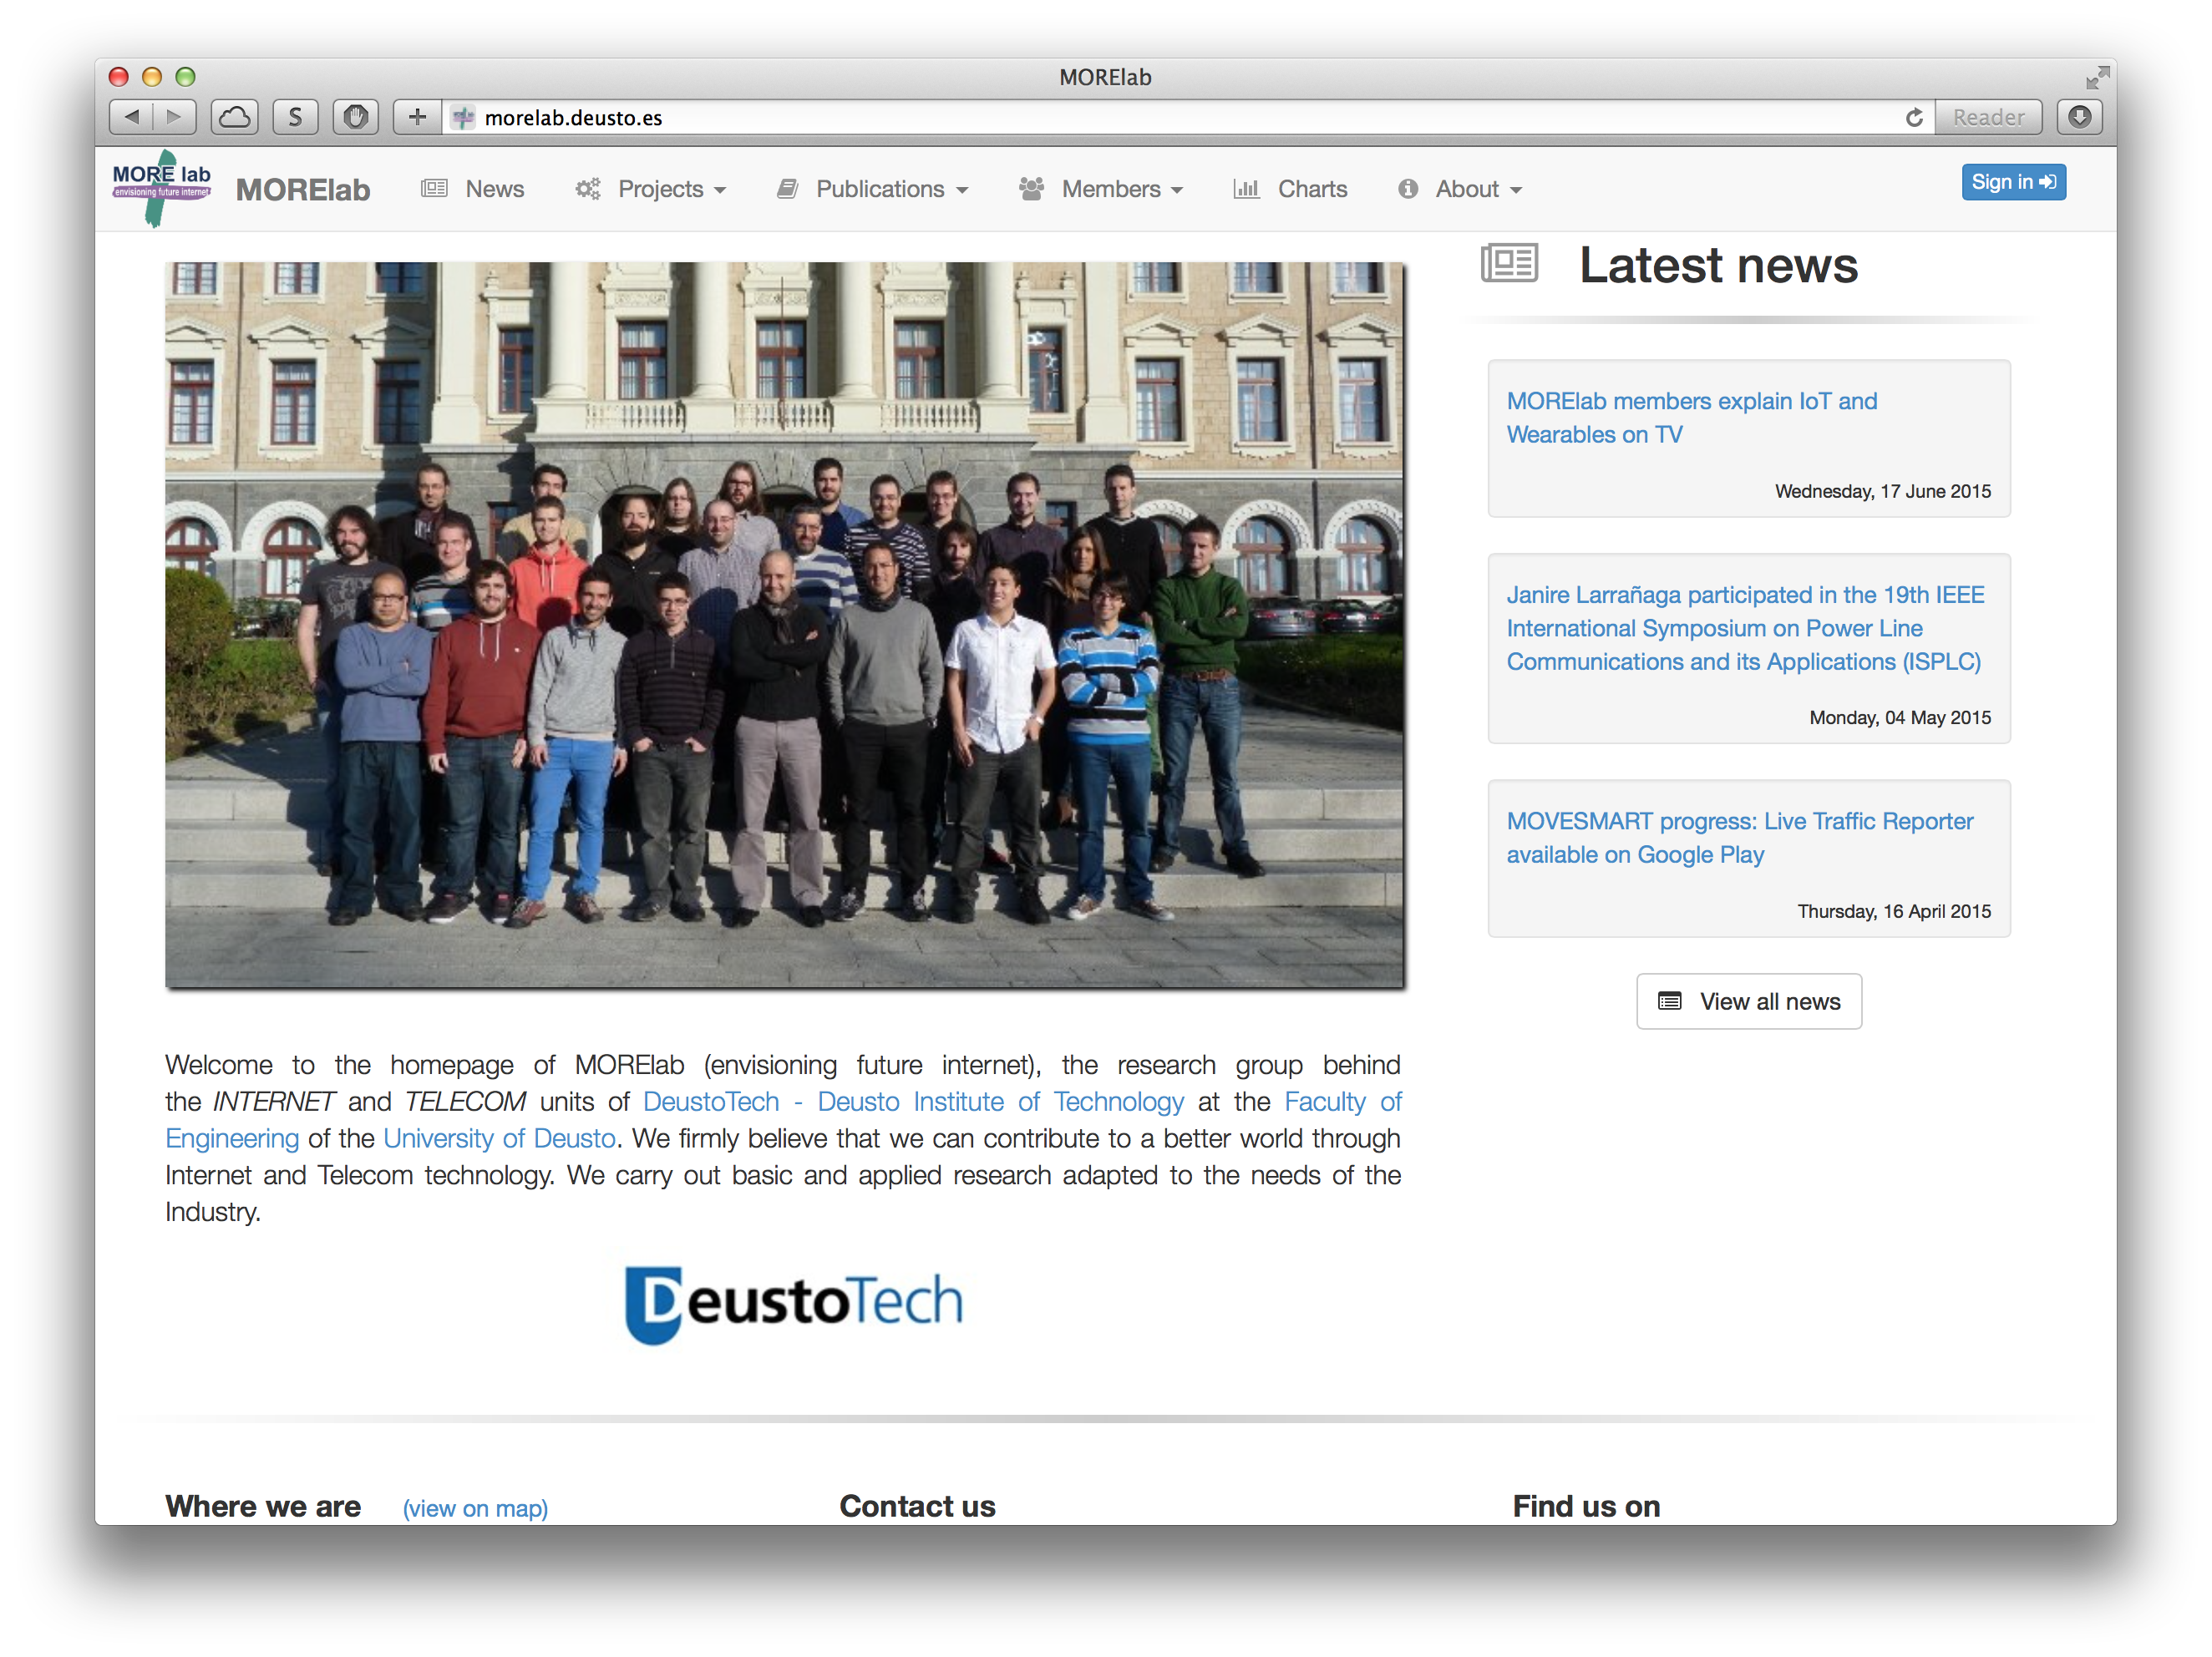
\includegraphics[scale=0.31]{fig/morelab_homepage}
	\caption{Página principal de \acrshort{labman} del equipo MoreLab}
	\label{fig:morelab_homepage}
\end{figure}

Este manual se centra en las opciones de \textit{Projects} y \textit{Publications}, dado que estas son las facetas en las que se ha trabajado a lo largo del proyecto y el resto están fuera del alcance.

\subsection{Projects: Buscador de proyectos de LabMan}

Esta página muestra en principio la lista de todos proyectos que involucran a los miembros del equipo de investigación sin filtrar. Mediante la barra de búsqueda sencillas (véase la figura \ref{fig:project_search_bar}), permite filtrar los proyectos por título o por el nombre del investigador que participe en los mismos.

\begin{figure}[!htbp]
	\centering
	
\includegraphics[scale=0.4]{fig/search_bar}
	\caption{Barra de búsqueda de consultas simples}
	\label{fig:project_search_bar}
\end{figure}